% ULaTeX2e, calling the article.cls class and 12-point type.

\documentclass[12pt]{article}

% My packages

\usepackage{graphicx}
\usepackage{amsthm}
\newtheorem{mydef}{Definition}
\usepackage{dcolumn}
\usepackage{multirow}
\usepackage{booktabs}
\newcolumntype{d}{D{.}{.}{4.0}}
\newcolumntype{s}{D{.}{.}{1.4}}

% Users of the {thebibliography} environment or BibTeX should use the
% scicite.sty package, downloadable from *Science* at
% www.sciencemag.org/about/authors/prep/TeX_help/ .
% This package should properly format in-text
% reference calls and reference-list numbers.

\usepackage{scicite}

% Use times if you have the font installed; otherwise, comment out the
% following line.

\usepackage{times}

% The preamble here sets up a lot of new/revised commands and
% environments.  It's annoying, but please do *not* try to strip these
% out into a separate .sty file (which could lead to the loss of some
% information when we convert the file to other formats).  Instead, keep
% them in the preamble of your main LaTeX source file.


% The following parameters seem to provide a reasonable page setup.

\topmargin 0.0cm
\oddsidemargin 0.2cm
\textwidth 16cm 
\textheight 21cm
\footskip 1.0cm


%The next command sets up an environment for the abstract to your paper.

\newenvironment{sciabstract}{%
\begin{quote} \bf}
{\end{quote}}


% If your reference list includes text notes as well as references,
% include the following line; otherwise, comment it out.

\renewcommand\refname{References and Notes}

% The following lines set up an environment for the last note in the
% reference list, which commonly includes acknowledgments of funding,
% help, etc.  It's intended for users of BibTeX or the {thebibliography}
% environment.  Users who are hand-coding their references at the end
% using a list environment such as {enumerate} can simply add another
% item at the end, and it will be numbered automatically.

\newcounter{lastnote}
\newenvironment{scilastnote}{%
\setcounter{lastnote}{\value{enumiv}}%
\addtocounter{lastnote}{+1}%
\begin{list}%
{\arabic{lastnote}.}
{\setlength{\leftmargin}{.22in}}
{\setlength{\labelsep}{.5em}}}
{\end{list}}


% Include your paper's title here

\title{Hysteresis in human computation:\\ how one task affects another} 


% Place the author information here.  Please hand-code the contact
% information and notecalls; do *not* use \footnote commands.  Let the
% author contact information appear immediately below the author names
% as shown.  We would also prefer that you don't change the type-size
% settings shown here.

\author
{Edward Newell, Derek Ruths,\\
\\
\normalsize{\texttt{edward.newell@mail.mcgill.ca}}\\
\normalsize{\texttt{druths@networkdynamics.org}}\\
\normalsize{School of computer science, McGill University,}\\
\normalsize{3630 rue University, Montreal, Quebec, H3A 0C6, Canada}\\
\\
}

% Include the date command, but leave its argument blank.

\date{}



%%%%%%%%%%%%%%%%% END OF PREAMBLE %%%%%%%%%%%%%%%%



\begin{document} 

% Double-space the manuscript.

\baselineskip24pt

% Make the title.

\maketitle 



% Place your abstract within the special {sciabstract} environment.

\begin{sciabstract}

Microtask platforms combine the efforts of large numbers 
of people to perform tasks that are difficult to automate with computers 
alone.  These platforms support near-real-time task completion, mimicking a
compute server, and fundamentally shift the role of the human from consumer to 
producer of computing resources.  To realize its full
potential, we must understand how human computation differs from machine 
computation, and address the biases known to be inherent in 
human cognition.  The effects of various task-design variables on worker
performance have been investigated, but there has been little 
investigation into how consecutive tasks influence one another. Here we show 
that the responses in later tasks are strongly influenced by the content of 
earlier ones, an effect that is as strong or stronger than the effect of 
framing.  Our findings are not solely cautionary; we find
that these \textit{intertask effects} can be harnessed to improve the quality 
of responses, and thereby help to achieve expert-level judgments in citizen 
science and other crowdsourcing initiatives. 
As an ancillary contribution, we demonstrate the use of machine learning 
algorithms measure exposure-induced human bias, in terms of its ability to 
influence human computations. 
\end{sciabstract}

\section*{Introduction}
Microtask crowdsourcing platforms like Amazon Mechanical Turk (MTurk) make it 
possible for requesters to submit batches of tasks to a large pool of 
workers, who do the tasks for fun, a sense of purpose, and remuneration 
\cite{kazai2013analysis,Antin20122925}.  
Typical tasks include tagging and categorizing images 
\cite{6116320,Zhai2012357}, transcribing voice recordings 
\cite{chandler2013breaking,paolacci2010running}
or handwritten notes \cite{Berinsky2012351,Finnerty2013}, and judging the 
relevancy of search results 
\cite{le2010ensuring,grady2010crowdsourcing,alonso2009can,kazai2013analysis}.
Originally used to distribute clerical work, these platforms 
increasingly serve as a means to engage experimental participants in a 
research 
setting \cite{paolacci2010running,Berinsky2012351,snow2008cheap,alonso2009can}.
This trend has seeded considerable interest in characterizing the parameters
of task design, and validating the microtask platform methodology (\#).

Computer scientists view microtask platforms in the context of general
computation.  In this regard, the platforms enable a tight integration of 
human and machine computation.  Researchers coined the term HPU 
(Human co-Processing Unit) in analogy to CPUs and GPUs \cite{5543192}.  
Ongoing research pursues the establishment of an HPU instruction set
including basic operators like \texttt{vote}, \texttt{subdivide}, \texttt{map},
\texttt{reduce}, \texttt{sentiment}, and \texttt{image\_tag} (\#).  Libraries 
are being developed to give the programmer more seamless access to HPU 
resources 
 \cite{little2010turkit,minder2011crowdlang,minder2012crowdlang,kittur2011crowdforge}.  
As with other architectures, the HPU architecture makes entirely new classes 
of problems tractable for the programmer (\#).

But the ability to program with high-level human instructions comes with a 
cost: HPU output is inherently noisy.  Part of this noise can be explained
in terms of worker demography (\#).  But systematic cognitive biases also 
play a role (\#), a dimension of variability we investigate here.   
So far, investigation has explored such design factors as the level of 
pay \cite{kazai2013analysis}, training \cite{le2010ensuring}, pre-screening of 
workers \cite{paolacci2010running}, and user-interface design 
\cite{Finnerty2013}.  Researchers have also investigated \textit{framing}, 
by testing the effects of describing the workflow context 
\cite{Kinnaird2012281}, the purpose of tasks 
\cite{chandler2013breaking}, or using alternate problem descriptions
\cite{thibodeau2013natural}.  To our knowledge, no study has investigated 
the influences that consecutive microtasks exert on one another.

It is known that people are susceptible to priming effects 
\cite{BJOP1796,No2007,beller1971priming}, and, in particular, task-repetition 
effects \cite{Gass1999549,sohn2001task}.  Thus, a worker's response during
one task may depend in part on previous ones.  Such \textit{intertask} effects
would amount to a kind of \textit{hysteresis}, meaning that HPU outputs are not
only a function of the current input, but also of the history of inputs, with
important implications for the design of crowdsourcing initiatives.

Here we describe a series of experiments using the Amazon Mechanical
Turk (MTurk) microtask platform in which we studied intertask effects
for image-labeling tasks.  Image-labeling tasks are among the most 
common kinds of microtasks
\cite{chandler2013breaking,Berinsky2012351,Finnerty2013,paolacci2010running}, 
and it seems likely that this will remain the case in the long term because
they provide a source of ground truth in computer vision research 
\cite{5543192}.  
During the experiments, workers were presented with a series of images (one at
a time), and had to provide five descriptive words (\textit{labels}) for each.
We varied first five images (hereafter the \textit{initial tasks})
and observed the effect this had on the workers' labels for the last five
(\textit{test tasks}).

The initial tasks were chosen to embed a certain \textit{prime concept}.
In our first experiment, our prime concepts were \textit{food} and (non-food) 
\textit{objects}.  In our second experiment, the prime concepts were 
\textit{food} and \textit{culture}.  The test tasks for the experiments used 
images that combined both prime concepts. Any given worker performed in only 
one experiment, and was randomly assigned initial tasks based on one of the 
prime concepts.  From the perspective of the worker, we made no distinction 
between the initial tasks and test tasks.

As a point of comparison, we included treatments in which we induced
\textit{framing}.
In the framing treatments, before workers begin the tasks, we told them that 
the purpose of study was to understand the visual perception of 
``food and ingredients'' in one case, or the 
perception of ``objects and tools'' in another.  We varied the language of 
the framing text (hereafter simply the \textit{frame}), and experimented with 
requiring the worker to echo the frame using a combo-box input.

We found that intertask effects were stronger than framing, unless the worker
was required to echo the frame, in which case both exposures were on par.  
Our results demonstrate that initial tasks can change 
workers' focus in later tasks.  We also found that intertask effects 
significantly altered the level of specificity, and the diversity of 
vocabulary that workers used, and did so in ways that differed from framing.
Contrary to our initial expectations, our findings suggest that the HPU 
programmer can leverage intertask effects.  By carefully designing workflows,
worker focus, specificity, and expressivity can be tuned.  Our 
findings carry two lessons for the task designer: intertask
effects can severely bias HPU output if uncontrolled, but if properly 
controlled, intertask effects might be optimized, which may be of significant 
utility in achieving expert-level output.

\paragraph*{Measuring computational hysteresis.}
Before describing the details of our experiments, we explain some 
choices made in measuring intertask and framing effects 
(hereafter collectively \textit{exposure effects}).  
It might be tempting to invoke the concept of a ``neutral frame of mind'' 
which would serve as a baseline for drawing comparisons.  But such a concept 
seems both difficult to define, and unlikely to arise.
Therefore, we instead always consider the effect of one exposure 
\textit{relative} to another.  Thus, our experiments consist of 
pairs of treatments between which we can make meaningful comparisons.

Our goal in measuring exposure effects is to show that they can actually 
alter the course of algorithms.
We could, by means of a $\chi^2$ test, reject the null hypothesis that
differently exposed HPUs have the same distribution of outputs.
However, this alone would not demonstrate a practically significant effect, in 
terms altering the execution path of algorithms.

For this reason, we develop a measure in which we train classifier algorithms 
to infer the exposure of an HPU from its outputs.
If a classifier infers an HPU's exposure with significantly 
better accuracy than provided by chance, then the HPU outputs must have 
been affected by the exposure.  
But in addition, the classifier serves as a kind of certificate, since it is 
an example of an algorithm whose path of execution is influenced by the 
exposure of 
individual HPUs.  In the supplementary material, we ground our approach 
rigorously in terms of the L1-distance metric, which is a measure of 
divergence between distributions.  The L1-distance ranges from 
0 to 1.  In our case, a value of 1 indicates that the HPU's exposure
influences its output so strongly that the exposure can be inferred from the
output without ambiguity.  A value of 0 indicates that the exposure has no
impact on the HPU's outputs.  The connection between the
L1-distance, $D_\mathrm{L1}$, and a classifier's accuracy, $\eta$, is given by:
\begin{equation}
	D_\mathrm{L1} \geq 2 \eta - 1, 
	\label{l1}
\end{equation}
Since a classifier's performance provides a lower bound on the L1-distance, 
we shall denote $D_\mathrm{L1}^-\equiv 2\eta-1$.
The L1-distance admits the following interpretation: if two distributions
$P$ and $Q$ have an L1-distance $d$, then in the worst case, the 
frequency with which a binary algorithm operating on samples
from $P$ outputs a 1, will differ from that when operating on samples from 
$Q$ by $d \times 100\%$.  
Thus, we can interpret $D_\mathrm{L1}^-$ as a kind of
lower bound for the worst-case bias induced by HPU hysteresis.
We provide further discussion of the statistical properties of our approach 
in the supplementary material.

\paragraph{Experimental setup.}
\begin{figure}
	\centering
	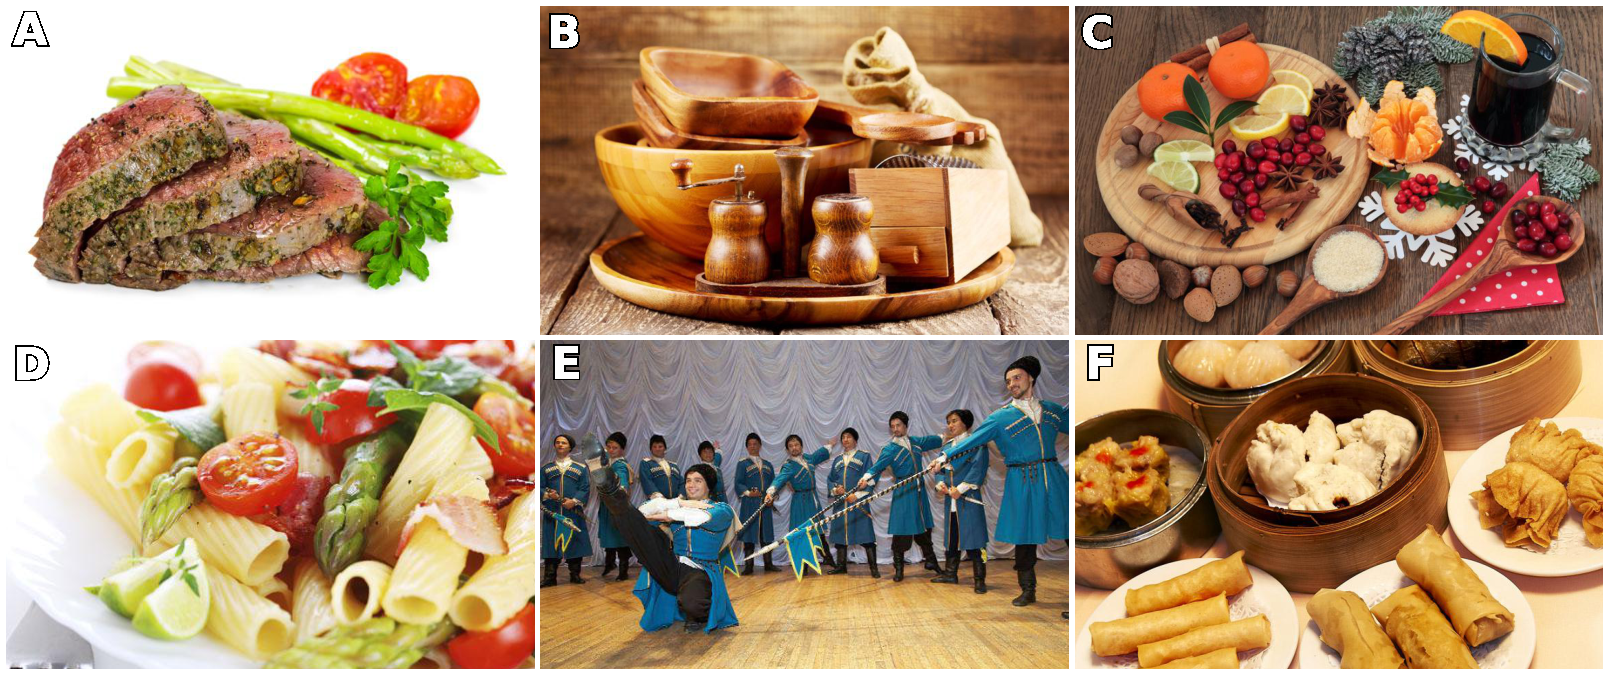
\includegraphics[scale=0.7]{figs/images.jpg}
	\caption{
		Examples of images used in labeling tasks. Images from initial
		tasks: A) \textit{task1:food}, B) 
		\textit{task1:obj}, D) \textit{task2:food}, 
		E) \textit{task2:cult}.  Images from  test tasks: C) \textit{exp1}, 
		F) \textit{exp2}.  The full set of experimental materials is 
		shown in the supplementary material.
	}

	\label{fig:task}
\end{figure}
We performed two experiments, soliciting respectively 2300, and 900 MTurk 
workers to label images depicting food, kitchen- and dining-ware, and cultural
scenes.  In a given experiment, all workers performed the same test
tasks, the output of which was our main dependent variable.  Before performing
the test tasks, workers were subjected to an exposure, via one of 
two \textit{modalities}: either they completed a set of initial tasks, or 
were exposed to a frame, or both.  As mentioned, from the perspective of the worker, 
there was no distinction or discontinuity between initial and test tasks.

We organized the experiments into \textit{treatment pairs}.  Both treatments in a 
pair involved the same exposure modality, but differed in the
content of the exposure.  In Table 1, we summarize the various experimental
treatments, and introduce a naming convention that we use to refer to 
treatments and treatment pairs.
In the treatment pairs that studied intertask effects (\textit{task1} and
\textit{task2}), workers performed 10 image-labeling tasks, with the first 
five tasks comprising the initial tasks and the last five tasks comprising the
test tasks.

In the first experiment, the content of the exposures was based on the prime
concepts \textit{food} and \textit{objects} (throughout, ``objects'' should be
taken to imply ``non-edible objects'').  So, 
in \textit{task1:food}, the initial tasks contained images depicting food, 
while in \textit{task1:obj}, they contained images depicting objects, 
including kitchen and dining-ware (see Fig~\ref{fig:task}).  Meanwhile, 
for the exposures in \textit{frame1} we indicating that the study was
``funded by the laboratory for the visual perception of \{ Food and Ingredients
$\vert$ Objects and Tools~\}''.  To further strengthen the frame, we 
introduced another pair of framing treatments, \textit{echo}, with stronger
wording: ``The purpose of this study is to understand the visual perception
of \{ Food and Ingredients $\vert$ Objects and Tools~\}'', and required
the worker to echo the purpose of the study by selecting it among other 
options in a combo-box input.

Note that food and objects are both relatively well-defined classes of 
physical entities.  To explore a different conceptual axis, in 
\textit{exp2} we adopted the prime concepts food and \textit{culture}.
Compared to food and objects, culture is more abstract, difficult to define, 
and, rather than comprising a class of physical entities, it encapsulates
sets of beliefs, values, and practices.  Examples of images from the initial 
tasks in \textit{task2} are shown in Fig.~\ref{fig:task}, and the full 
collection of 
experimental materials is presented in the supplementary material.  We 
ensured that workers only participated in one treatment of one experiment.

\setlength{\tabcolsep}{3pt}
\begin{table}[t]
\centering
\begin{tabular}{ c c c c c }
		\hline \noalign{\smallskip}
		\multicolumn{3}{c}{\textbf{Treatment name}} & \parbox[c]{1.6cm}{\centering \textbf{Framing\\ Prime}} & \parbox[c]{1.7cm}{\centering \textbf{Initial\\ image set}}	\\ 

		\noalign{\smallskip} \hline \noalign{\smallskip}

		\multirow{6}{*}{ \parbox[c]{1cm}{ \phantom{XXX} exp1}} 
			& \multirow{2}{*}{task1} & food & none & food\\
			& & obj & none & objects\\

			\noalign{\smallskip} \cline{2-5} \noalign{\smallskip}
			& \multirow{2}{*}{frame1} & food & food & none\\
			& & obj & objects & none\\

			\noalign{\smallskip} \cline{2-5} \noalign{\smallskip}
			& \multirow{2}{*}{echo} & food & food & none\\
			& & obj & objects & none\\

		\noalign{\smallskip} \hline \noalign{\smallskip}

		\multirow{4}{*}{exp2} 
			& \multirow{2}{*}{task2}  &  food & none & food\\
			& 	&  cult & none & culture\\
			\noalign{\smallskip} \cline{2-5} \noalign{\smallskip}
			& \multirow{2}{*}{frame2} & food & food & food\\
			& 	& cult & culture & food\\

		\noalign{\smallskip} \hline  
	\end{tabular}

	\caption{ \footnotesize{ 
		We use the treatment names shown to refer to specific sections of 
		the data collected.  For example, \textit{task2:food} refers to the
		treatment in the second experiment which was not exposed to a frame, 
		and whose initial tasks contained images of food (7th row).
	}}
	\label{table:1}
\end{table}



\paragraph{The strength of intertask effects.}

We assessed the strength of intertask and framing effects
by training a multinomial naive Bayes classifier to infer a worker's exposure
based on the labels provided in the test tasks (see Fig.~\ref{fig:theta}).
This inference was made over the two possibilities given the treatment pair
to which the worker had been assigned.
We found that in \textit{task1}, whether a worker performed food- or 
object-containing initial tasks, had a strong effect on their subsequent 
labels, introducing a bias that probably exceeds 30\%.  In comparison, the 
framing effect in \textit{frame1} did 
not influence workers' labels enough for the classifier to make predictions 
with significantly better accuracy than that afforded by chance.  The results 
for \textit{exp2} show a similar, but even more pronounced trend, with the bias
induced by intertask effects in \textit{task2} probably exceeding 50\%.

We see a comparable effect size in the \textit{echo} treatment pair.
We expected \textit{echo} to show a very strong effect because, by requiring
the worker to echo the purported purpose of the task, we signal that it
is of particular importance, more so than the instructions provided
beforehand.  The fact that the intertask effects were on par with the framing 
effects in \textit{echo} shows just how powerful intertask effects can be.

\begin{figure}
	\centering
	\includegraphics[scale=1]{figs/theta.pdf}
	\caption{
		Lower-bound estimates for the  worst-case bias introduced in image
		labeling tasks due to worker exposure effects.  The estimate was 
		based on the performance of a multinomial naive Bayes classifier,
		trained to infer an HPUs exposure. A) bias induced through various
		modalities and prime concepts (see Table 1). B) Bias induced in 
		\textit{task1}, as a function of test task position.  Error bars
		show the one-tailed 95\% confidence interval.
	}
	\label{fig:theta}
\end{figure}

\paragraph{Dynamics of intertask effects.} It is natural to expect 
intertask effects to attenuate as a worker proceeds through test tasks.  
In \textit{task1}, we permuted the test tasks, allowing us to 
measure intertask effects as a function of test task position, while factoring
out the content-dependant differences between test tasks
(see Fig.~\ref{fig:theta}B). 
We found intertask effects were most pronounced for the first test image,
dropping off substantially for the second test task, but maintaining a 
significant effect through until the 5th test task.  
This shows that the range of intertask effects extend accross at least 5 
tasks, and probably substantially more.
This makes intertask effects of greater concern, but as we will show, it also
makes intertask effects of greater potential utility.
In future work, it would be interesting to investigate whether a worker's
susceptibility to intertask effects varies accross a large batch.  For example,
It is conceivable that the first few tasks induce especially strong
or long-lasting effects, in effect ``setting the tone'' for the rest of the batch.

\paragraph{Detailed influences on worker outputs.} 
\begin{figure}
	\centering
	\includegraphics[scale=1]{figs/vocab_specificity.pdf}
	\caption{
		Detailed exposure effects on workers label vocabulary, for various
		exposure modalities and prime concepts (see Table 1).  A) Change in 
		the number of food-related labels used. B) Change in the total number 
		of \textit{unique} food-related labels used. C) Relative specificity
		of treatment pairs, when considering food-related labels.  For all
		plots, a positive bar height indicates an increase for the 
		food-exposed treatment.
	}
	\label{fig:specificity}
\end{figure}

Having observed significant effects from framing and task-exposure,
we looked in greater detail at the nature of the effects.  For instance,
does a food-oriented exposure induce workers to provide more food-related
labels?  And if so, does this explain the classifier's ability to distinguish
a worker's initial exposure? 

To answer these questions, we used the wordnet corpus, augmented with names of
ethnic foods learned from the Internet.  Wordnet provides a (roughly)
hierarchical set of relationships between nouns, called hypernym-hyponym
relationships.  A hypernym is a generalization, while a hyponym is a 
specialization.  So, for example, ``bread'' is hypernym to ``rye bread'' 
and hyponym to ``baked goods''.

Using an augmented hypernym-hyponym structure of wordnet to identify nouns 
depicting food, we found that, for the experimental pairings in 
\textit{exp1}, the
food-exposed treatments did produce a significantly larger fraction of 
food-related labels (see Fig.~\ref{fig:specificity}A).  While the shift in 
focus with regard to food does help explain the classifier's ability to 
infer workers exposure, it still leaves most of this difference unexplained 
(*).
Furthermore, such a simple relationship cannot explain the observation for
\textit{exp2:task2} where we see a significant but reversed effect
(see Fig.~\ref{fig:specificity}A).
Given the difference between the food-culture and food-object axes, it should
not be surprising that the effect of exposure is different.  We must therefore
be prepared to accomodate multiple, countervailing factors which influencing 
the bulk number of references to the prime concept (food).  We will come back 
to this notion momentarily.

To explore these effects further, we looked more closely at which particular
labels are most suppressed (activated) by a worker's exposure.  Remarkably,
we found that, for all treatment pairs, ``food'' was always the most 
suppressed label among 
the food-exposed workers.  This is surprising, considering 
that the bulk incidence of food-related labels mostly \textit{increased} among 
food-exposed workers.  But taken together, the increase in references to food 
and the decrease in the incidence of ``food'' per se (which is the most generic
food-reference in the wordnet-based ontology), necessarily implies that
food-exposed workers have traded ``food'' for more specialized references to 
food. 

In a crowdsourcing task, considerable effort must be given to shaping the 
vocabulary with which a worker engages a task.  To draw an example from the 
domain of citizen science, in galaxy zoo, workers catalog images of galaxies 
in terms of smoothness, and the presence of rings, dust lanes, digital 
disturbances, and so on.  Shaping this vocabulary is crucial to the reliability
of results.  In galaxy zoo, the interface contstrains and prompts the user
with this basic vocabulary.  But this would not appear to be sufficient, since
a set of positive and negative training examples are used, together with
peer-to-peer and peer-to-expert exchange in discussion areas, presumably to
refine and homogenize the vocabulary (\#).  

In our set-up, where the worker's vocabulary is unconstrained, we can 
directly observe the effects that frames and initial tasks have on worker 
vocabulary.  By looking at the number of unique food-related labels that 
workers produced, we assessed the richness of vocabulary that workers used when
referring to food (see Fig.~\ref{fig:specificity}B.  We found that the 
food-exposed workers use a richer vocabulary of 
food-related words, even in cases like \textit{task2:food}, where they 
made fewer references to food overall.  
Interestingly, task-based exposure to food had a stronger enriching effect 
(for food-vocabulary) than did framing-based exposures. (* explain why vocab 
diversity is useful.) 

Using the ontology of food induced by wordnet, we were able to directly
calculate the relative specificity of workers from different treatments.
To do this, we considered all the labels from one treatment
(for example \textit{task1:food}) and compared these to all the labels from 
another (\textit{task1:obj}).  For all possible comparisons, we observed 
which treatment's label was more specific more often, and normalized this
quantity as a percentage (we provide greater detail in the supplementary 
material).

We calculated the relative specificity for all treatment pairs, while 
restricting focus to 
food-related labels (see Fig.~\ref{fig:specificity}C).  We found that 
the food-exposed workers always provided food-references of substantially 
greater specificity.  Workers that had labeled images containing food 
were about 12\% more specific than those that labeled images of objects,
and about 20\% more specific than those that labeled images of cultural 
scenes.  With respect to the specificity of food references, framing effects 
were on par with intertask effects.

Taken together, the results presented in Fig.~\ref{fig:specificity} can 
be explained by a combination of priming and a context-dependant appraisal
of salience resembling \textit{negative} priming.
Negative priming occurs when a repeated stimulus, which is perceived to be
non-salient, begins to be ignored.  

We propose that, as a worker from \textit{task1:food} proceeds through the 
initial tasks, food-related memories and concepts are activated, increasing 
the likelihood that she uses a variety of food-related labels.  This accounts
for the overall increases the number of food-related labels, as well as the 
richness and specificity of her food-related vocabulary.  At the same time,
the fact that the images contain food at all begins to appear non-salient 
since due to its constancy, suppressing the most generic labels, such as 
``food''.  Thus, there is a simultaneous emphasis of the specialized 
references to the prime concept and de-emphasis of generic references. 

This view accounts for the observation that there are fewer
food-related references overall in \textit{task2:food} compared to 
\textit{task2:cult}.  Workers in \textit{task2:food} are primed to use
specialized food references and negatively primed against using generic
ones.  Then, when workers encounter images with much more prominent 
cultural content in the test tasks, they attends to this novel content, 
decreasing the balance of food references.  
Meanwhile, workers in 
\textit{task2:cult} experience novelty from the introduction of food-oriented 
content, and, attending to it, drive the relative difference in the quantity 
of food-related labels further negative in in Fig.~\ref{fig:specificity}A.

Based on these observations, we submit the following ideas for consideration 
by the designers of crowdsourced initiatives.
\begin{enumerate}
	\item{
		Training tasks should be preferred over examples, since the immediate
		active use of information appears to increase its impact.
	}
	\item{
		Training tasks should contain the same distribution of 
		noise (or ``distracting features''), as the real dataset.
		Exposing workers to irrelevant features and identifying them as such
		will help direct focus toward salient features by virtue of
		negative priming.
	}
	\item{
		\textit{Validation tasks}, for which the correct output is known,
		are often used as a quality control measure.
		These should be dually considered as \textit{calibration tasks}, and
		should be designed to help worker to maintain an optimally primed 
		state. Feedback, for both correct and incorrect responses, 
		may further reinforce salient features.
	}
	\item{
		In many applications, such as the detection of pre-ictal 
		(pre-seizure) EEG traces, workers encounter few positive examples
		(most traces are not pre-ictal).  In the absence of positive examples,
		the target concept may degrade or drift.
		Drawing calibration tasks drawn from the underrepresented class may 
		help sustain the target concept.
	}
	\item{
		For the most precise classifications, it may be helpful to
		begin with a coarse classification.  For example, workers could 
		initially choose from  \texttt{class 0}, \texttt{class 1}, and 
		\texttt{borderline}.  Following the coarse classification, the 
		\texttt{borderline} examples could be batched together, allowing 
		workers to focus on finer distinctions which are only salient for fine 
		distinctions.
	}
\end{enumerate}

These techniques follow logically from our observations, but they are educated 
guesses.  We leave their direct testing to future work.

\paragraph{Conclusion.}
Our results show that intertask effects are 
as strong as framing effects, and are stronger when the frame is not echoed.
Our analysis using wordnet reveals that intertask and framing effects
act on workers' vocabulary in subtle ways.  Both exposure modalities 
increased the richness of workers' vocabulary in reference to the prime 
concept, but more so in the case of task-based exposure.  Both modalities 
also increased the specialization of workers' vocabulary in reference to the 
prime concept.

We recommend that intertask effects be considered when designing crowdsourced
studies.  Despite efforts to eliminate biases from the context of tasks,
the greatest source of biases may lurk in the tasks themselves.
At the same time, their positive effects on workers' vocabulary suggests 
that, when properly controlled, intertask effects may be
used to optimize HPU performance.  Based on the enriching effects we observed
for worker vocabulary, intertask effects might be leveraged to achieve 
expert-level annotation in a wider variety of applications.

\bibliography{newbib}
\bibliographystyle{Science}


\section*{Supplementary Material}

\subsection*{Assessing task similarity}
\begin{table}
\centering
\begin{tabular}{ l  s s s s}

\toprule    
Image set   
& \multicolumn{1}{c}{Ambig.} 
& \multicolumn{1}{c}{Cultural} 
& \multicolumn{1}{c}{Ingr.}
& \multicolumn{1}{c}{Test} \\
  
\midrule

Ambiguous  & 1 & 0.0418 & 0.142 & 0.167 \\

Cultural  & 0.0418  & 1 & 0.0347 & 0.0561 \\

Ingredients  & 0.142  & 0.0347 & 1 & 0.110 \\

Test & 0.167  & 0.0561 & 0.110 & 1
\\
\bottomrule

\end{tabular}
\caption{\footnotesize{
Pairwise similarities of each image set based on the labels attributed to them (see \textbf{Eq. 4}).
}}
\label{table:2}
\end{table}

One weakness of the above analysis is the reliance on the informal notion
of the similarity of one set of images to another. The 
characterization of image content is a deeply complex issue that has been 
approached by many disciplines \cite{panofsky1939studies,shatford1986analyzing,Tversky1977327,Jaimes20002}. \textit{Perceptual similarity} is a 
particularly recalcitrant concept.   But to formalize our claim, we seek a 
measure of similarity between two sets of images, 
\textit{with respect to the labeling task}.  This can be operationalized
in a straightforward way, by using the similarity of the labels given to images
as a proxy for the similarity of the images.  Thus, to measure the 
similarity between two sets of images, X and Y , we computed the Jacquard 
index between the sets of labels attributed to them:
$$
	\mathrm{Sim}(X,Y) = \frac{L(X) \cap L(Y)}{L(X) \cup L(Y)}
$$
where $L(X)$ denotes the set of labels attributed to images in $X$.

The pairwise similarities of the image sets are presented in Table 2. This 
shows that the workers that yielded higher specificity labels were from 
treatments whose initial tasks were more similar to the test tasks (c.f.
\textbf{Fig 3}).

Such a phenomenon would be consistent with the psychological mechanism known as
\textit{negative priming}.

\end{document}

